\chapter{Искусственные нейронные сети}
\section{Общее определение искусственной нейронной сети}

Искусственными нейронными сетями (ИНС) называется совокупность моделей биологических нейронных сетей.
ИНС представляет собой сеть искусственных нейронов, связанных между собой искусственными синаптическими соединениями.
Сеть обрабатывает входную информацию и в процессе изменения своего состояния во времени формирует совокупность выходных сигналов.\cite{COURSE}
Так как ИНС моделирует реальную нейронную сеть, рассмотрим принципы функционирования биологического образца.
Структурной единицей биологической нейронной сети является нейрон (нервная клетка).
\begin{figure}[h]
\center{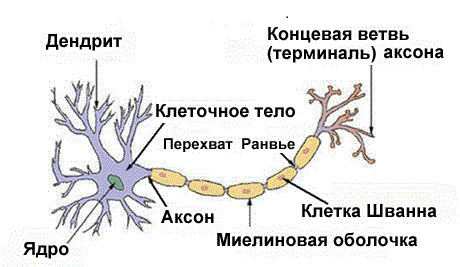
\includegraphics{Neuron.png}}
\caption{Структура нейрона}
\label{ris:neuron}
\end{figure}
Нейрон (рис.~\ref{ris:neuron}) является особой биологической клеткой, корорая обрабатывает информацию.
Она состоит из тела клетки, или сомы, и двух внешних древоподобных ветвей: аксона и дендритов.
Тело клетки включает ядро, которое содержит информацию о наследственных свойствах, и плазму, обладающую молекулярными средствами для производства необходимых нейрону материалов.
Нейрон получает сигналы (импульсы) от других нейронов через дендриты и передают сигналы, сгенерированные телом клетки, вдоль аксона, который в конце разветвляется на волокна.
На окончаниях этих волокон находятся синапсы. 
Синапс является элементарной структурой и функциональным узлом между двумя нейронами (волокно аксона одного нейрона и дендрит другого).
Когда импульс достигает синаптического окончания, высвобождаются определенные химические вещества, называемые нейротрансмиттерами.
Нейротрансмиттеры диффундируют через синаптическую щель, возбуждая или затормаживая, в зависимости от типа синапса, способность нейрона-приемника генерировать электрические импульсы.
Результативность синапса может настраиваться проходящими через него сигналами, так что синапсы могут обучаться в зависимости от активности процессов, в которых они участвуют.
Эта зависимость от предыстории действует как память, которая, возможно, ответственна за память человека.
\cite{nn_int_jain}
Созданные из таких структурных элементов биологический нейронные сети обладают следующими свойствами:
\begin{itemize}
\item[-] {\bfПараллельность обработки информации. }
Каждый нейрон формирует свой выход только на основе своих входов и собственного внутреннего состояния под воздействием общих механизмов регуляции нервной системы.
\item[-] {\bfСпособность к полной обработке информации. }
Все известные человеку задачи решаются нейронными сетями.
К этой группе свойств относятся ассоциативность (сеть может восстанавливать полный образ по его части), способность к классификации, обобщению, абстрагированию и множество других.
\item[-] {\bfСамоорганизация.}
В процессе работы БНС самостоятельно, под воздействием внешней среды, обучаются решению разнообразных задач.
Неизвестно никаких принципиальных ограничений на сложность задач, решаемых БНС.
Нервная система сама формирует алгоритмы своей деятельности, уточняя и усложняя их в течении жизни.
\item[-] {\bfНаждежность. }
Биологические НС обладают фантастической надежностью: выход из строя даже 10\% нейронов в нервной системе не прерывает ее работы. 
По сравнению с последовательными ЭВМ, основанными на принципах фон-Неймана, где сбой одной ячейки памяти или одного узла в аппаратуре приводит к краху системы.\cite{COURSE}
\end{itemize}

